% =============================================================================
% final_report.tex — BIOSTAT 629 Final Written Report
% Compile from the project root:
%   pdflatex final_report.tex   (run twice for cross-references)
% Requires: MiKTeX, TeX Live, or TinyTeX (tinytex::install_tinytex() in R)
% Figures read from:  docs/figures/
% =============================================================================

\documentclass[12pt]{article}

% ── Layout & spacing ──────────────────────────────────────────────────────────
\usepackage[margin=1in]{geometry}
\usepackage{setspace}
\doublespacing

% ── Math & text ───────────────────────────────────────────────────────────────
\usepackage{amsmath}
\usepackage{microtype}          % better line breaks
\usepackage{parskip}            % block paragraphs, no indent

% ── Tables ────────────────────────────────────────────────────────────────────
\usepackage{booktabs}
\usepackage{array}
\usepackage{multirow}

% ── Figures ───────────────────────────────────────────────────────────────────
\usepackage{graphicx}
\usepackage{float}
\usepackage{caption}
\captionsetup{labelfont=bf, font=small, skip=4pt}

% Figures live in docs/figures/ relative to the project root.
% Compile from the project root:  pdflatex final_report.tex
\graphicspath{{docs/figures/}}

% ── Links ─────────────────────────────────────────────────────────────────────
\usepackage[colorlinks=true, linkcolor=blue,
            citecolor=blue, urlcolor=blue]{hyperref}

% ── Title ─────────────────────────────────────────────────────────────────────
\title{%
  \textbf{Racial and Ethnic Disparities in Driver Gene Mutations\\
  and Overall Survival in Non-Small Cell Lung Cancer}\\[0.5em]
  \large BIOSTAT 629 --- Final Written Report%
}
\author{Kai Wei \\ Department of Biostatistics, University of Michigan}
\date{\today}

% =============================================================================
\begin{document}
\maketitle
\thispagestyle{empty}

% ── Abstract ──────────────────────────────────────────────────────────────────
\begin{abstract}
\noindent
Non-small cell lung cancer (NSCLC) is the leading cause of cancer
mortality in the United States, and racial and ethnic minorities experience
substantially worse outcomes than non-Hispanic White patients.
Whether survival gaps are mediated by differential frequencies of oncogenic
driver gene mutations remains unclear.
We analyzed 7,775 NSCLC patients from MSK-CHORD 2024 (cBioPortal) to test
whether driver gene mutation frequencies differ across racial/ethnic groups,
whether observed differences persist after multivariable adjustment, and
whether they partially mediate racial survival disparities.
Chi-square tests with Benjamini-Hochberg false discovery rate (BH-FDR)
correction identified significant race-mutation associations for six of eight
genes tested.
Multivariable logistic regression confirmed that Asian patients carry 2.93
times the adjusted odds of EGFR mutation compared with White patients
(95\% CI 2.43--3.53) after adjusting for smoking history, disease stage,
histologic subtype, sex, and age.
Cox proportional hazards modeling showed that EGFR mutation independently
predicts improved survival (HR 0.82, 95\% CI 0.74--0.91), but the
Race\,$\times$\,EGFR interaction was non-significant.
Replication in colorectal and breast cancer cohorts confirmed that EGFR
enrichment in Asian patients is specific to NSCLC.
These findings implicate lung-tissue-specific biological mechanisms,
rather than pan-cancer racial genomic patterns, as the primary driver of the
observed mutation frequency disparities.
\end{abstract}

\newpage
\setcounter{page}{1}

% =============================================================================
\section{Introduction}

Lung cancer causes approximately 125,000 deaths in the United States annually,
and NSCLC accounts for roughly 85\% of cases \cite{Siegel2023}.
Racial and ethnic minorities---particularly Black and Hispanic patients---
experience worse NSCLC outcomes than non-Hispanic White patients.
This survival gap arises from at least two distinct sources: differences in
access to treatment and differences in tumour biology.
Oncogenic driver gene mutations determine the dominant pathway of tumour growth
and, critically, determine eligibility for targeted therapies.
Patients carrying an activating EGFR mutation respond to EGFR tyrosine kinase
inhibitors (TKIs), which produce substantially higher response rates and
longer progression-free survival than cytotoxic chemotherapy \cite{Mok2009}.

Prior work has reported higher EGFR mutation prevalence among Asian patients
with NSCLC \cite{Shigematsu2005}, but most studies were limited to single
institutions or did not fully adjust for smoking history, which itself varies
substantially by race/ethnicity and is the dominant mutagen for KRAS and
STK11.
Whether race-mutation associations are direct biological effects or proxies
for differential smoking exposure remains unresolved.

We test four scientific hypotheses.
(H1)~Mutation frequencies for eight clinically actionable driver genes differ
across racial/ethnic groups before covariate adjustment.
(H2)~EGFR enrichment in Asian patients and KRAS/STK11 enrichment in White
patients persist after multivariable adjustment for smoking, stage, histology,
sex, and age.
(H3)~Racial survival differences are partially mediated by differential EGFR
prevalence, quantified through a Race\,$\times$\,EGFR interaction term in a
Cox proportional hazards model.
(H4)~The EGFR-race association is specific to NSCLC and does not replicate in
colorectal or breast cancer, where EGFR is not a dominant oncogenic driver.

% =============================================================================
\section{Data and Variables}

MSK-CHORD 2024 (Memorial Sloan Kettering Cancer Center Harmonized Oncology
Research Database and Cohort) was downloaded from cBioPortal in April 2024
\cite{Cerami2012}.
The dataset contains 25,040 patients sequenced with MSK-IMPACT, a targeted
panel covering 341--505 genes.
We restricted the primary analysis to NSCLC (ICD-O histology codes for
adenocarcinoma, squamous cell carcinoma, and related subtypes); colorectal
(CRC) and breast cancer sub-cohorts served as replication sets.

Eight driver genes were selected based on prevalence, clinical actionability,
and established role in NSCLC biology: EGFR, KRAS, TP53, STK11, KEAP1, RB1,
ERBB2, and MET.
Each gene was coded as a binary variable (1~=~any non-synonymous somatic
mutation; 0~=~wild-type or not sequenced).
Race and ethnicity were harmonised to five U.S. Office of Management and
Budget (OMB) categories: White (non-Hispanic), Asian, Black/African American,
Hispanic/Latino, and Other/Unknown.
A critical implementation detail required correcting an ordering error: patients
recorded as ``Non-Spanish; Non-Hispanic'' in the source ethnicity field contain
the substring ``Hispanic'' and must be classified as White before the general
Hispanic/Latino rule is applied.
Misapplying the classification order misassigned approximately 5,000 White
patients as Hispanic/Latino and produced a spurious EGFR association in
preliminary analyses.

The primary cohort required complete data on race/ethnicity, all eight
mutation indicators, smoking history, disease stage, histologic subtype, sex,
and age.
Applying these criteria yielded 7,775 NSCLC patients (Table~\ref{tab:demo}).
Smoking history was missing for 28.3\% of patients; a sensitivity analysis
using 20 multiply-imputed datasets (MICE; \cite{vanBuuren2018}) confirmed that
complete-case results were not materially biased.

% =============================================================================
\section{Statistical Methods}

\subsection{Association Tests}

For each of the eight driver genes, we tested whether mutation frequency
differed across the five racial/ethnic groups using a contingency table
approach.
A chi-square test of independence was applied when all expected cell counts
exceeded five; Fisher's exact test with 10,000 Monte Carlo simulations was
applied otherwise.
Because eight simultaneous tests were conducted, raw $p$-values were adjusted
using the BH procedure at a false discovery rate of $q = 0.05$
\cite{BH1995}.
This procedure controls the expected proportion of false discoveries among
rejected hypotheses and is less conservative than Bonferroni correction, which
controls the probability of any false rejection.
Effect size was measured by Cram\'{e}r's $V$, where values near 0.10, 0.30,
and 0.50 correspond approximately to small, medium, and large associations
\cite{Cohen1988}.

\subsection{Multivariable Logistic Regression}

To isolate the direct effect of race/ethnicity on mutation status after
controlling for confounders, we fit a separate binary logistic regression model
for each driver gene:
\begin{equation}
  \operatorname{logit}\!\left[P(\mathrm{MUT}_{g}=1)\right]
  = \beta_0
  + \beta_1\,\mathrm{RACE}
  + \beta_2\,\mathrm{SMOKING}
  + \beta_3\,\mathrm{STAGE}
  + \beta_4\,\mathrm{SEX}
  + \beta_5\,\mathrm{AGE}
  + \beta_6\,\mathrm{HIST}
\end{equation}
where HIST collapses histologic subtype into three categories
(adenocarcinoma, squamous cell carcinoma, other/NOS) to avoid complete
separation caused by rare subtypes.
White (non-Hispanic) was the reference group.
Firth penalised regression was applied when standard maximum likelihood failed
to converge.
Adjusted $p$-values used BH-FDR correction across all race-gene pairs.
Results are presented as adjusted odds ratios (ORs) with 95\% profile
likelihood confidence intervals.

\subsection{Survival Analysis}

We fit a multivariable Cox proportional hazards model for overall survival (OS):
\begin{equation}
  h(t\mid\mathbf{X})
  = h_0(t)\exp\!\left(\boldsymbol{\beta}^{\!\top}\mathbf{X}\right)
\end{equation}
The model included race/ethnicity, EGFR mutation status, a
Race\,$\times$\,EGFR interaction term, smoking history, disease stage, sex,
and age.
Tied event times were handled with Efron's method.
The proportional hazards assumption was evaluated for each covariate using
Schoenfeld residuals (\texttt{cox.zph}); a significant global test ($p < 0.05$)
would indicate time-varying effects requiring model modification.
Kaplan-Meier (KM) curves were stratified by EGFR status, and the log-rank
test compared survival distributions.

\subsection{Replication}

The same logistic regression pipeline was applied to CRC and breast cancer
sub-cohorts from MSK-CHORD 2024.
Adjusted ORs from all three cancer types are displayed together in a single
forest plot to assess whether race-mutation associations are tissue-specific.

% =============================================================================
\section{Results}

\subsection{Cohort Characteristics}

Table~\ref{tab:demo} summarises the 7,775 NSCLC patients in the primary
analysis.
White (non-Hispanic) patients comprised 75.0\% of the cohort ($n = 5{,}830$),
followed by Asian ($n = 726$, 9.3\%), Hispanic/Latino ($n = 571$, 7.3\%), and
Black/African American ($n = 396$, 5.1\%).
Median age at diagnosis was 71 years (IQR 64--78).
Asian patients had the lowest smoking rate (35.3\% ever smokers) and the
highest Stage~IV proportion (53.7\%), while White patients had the highest
smoking rate (78.8\%).
Black patients were the youngest at diagnosis (median 67 years) and had the
second-highest Stage~IV rate (50.8\%).
All between-group differences reached $p < 0.001$ (Kruskal-Wallis for age;
chi-square for categorical variables).

\begin{table}[H]
\centering
\caption{Demographic and clinical characteristics by race/ethnicity
         ($n = 7{,}775$ NSCLC patients).
         All between-group differences $p < 0.001$.}
\label{tab:demo}
\begin{tabular}{lcccc}
\toprule
\textbf{Characteristic}
  & \textbf{White} ($n{=}5830$)
  & \textbf{Asian} ($n{=}726$)
  & \textbf{Black} ($n{=}396$)
  & \textbf{Hispanic} ($n{=}571$) \\
\midrule
Age, median [IQR]    & 72 [65, 78] & 68 [60, 76] & 67 [60, 74] & 70 [62, 78] \\
Ever smoker, \%      & 78.8        & 35.3        & 69.5        & 68.0        \\
Stage IV, \%         & 41.7        & 53.7        & 50.8        & 45.4        \\
Adenocarcinoma, \%   & 76.1        & 82.2        & 71.5        & 73.6        \\
\bottomrule
\end{tabular}
\end{table}

\subsection{Unadjusted Race-Mutation Associations}

Figure~\ref{fig:prev} shows mutation prevalence for all eight genes across
racial/ethnic groups.
EGFR shows the most pronounced disparity: Asian patients carry a 54.0\%
mutation rate versus 20.2\% in White patients and 26.8\% in Black patients.
KRAS and STK11 follow the reverse gradient, with White patients carrying the
highest rates (31.2\% and 14.5\%) and Asian patients the lowest
(9.8\% and 4.0\%).

Table~\ref{tab:chisq} presents BH-FDR-corrected association statistics for
all eight genes.
Six of the eight genes showed significant associations after correction.
EGFR had the largest effect size (Cram\'{e}r's $V = 0.229$,
$q = 3.0 \times 10^{-86}$), followed by KRAS ($V = 0.144$,
$q = 2.0 \times 10^{-33}$) and STK11 ($V = 0.097$,
$q = 1.3 \times 10^{-14}$).
MET ($q = 0.055$) and ERBB2 ($q = 0.109$) did not reach the $q = 0.05$
threshold.

\begin{table}[H]
\centering
\caption{Gene-race association tests in the NSCLC cohort ($n = 7{,}775$).
         BH-FDR correction applied across eight simultaneous tests at
         $q = 0.05$.
         Chi-square used when all expected cell counts $\geq 5$;
         Fisher's exact otherwise.
         Bold rows: $q < 0.05$.}
\label{tab:chisq}
\begin{tabular}{lccccr}
\toprule
\textbf{Gene}
  & \textbf{Test}
  & \textbf{Statistic}
  & \textbf{$p$-value}
  & \textbf{$q$-value (BH)}
  & \textbf{Cram\'{e}r's $V$} \\
\midrule
\textbf{EGFR}  & $\chi^2$ & 408.3 & $3.7\times10^{-87}$ & $\mathbf{3.0\times10^{-86}}$ & \textbf{0.229} \\
\textbf{KRAS}  & $\chi^2$ & 166.8 & $6.6\times10^{-35}$ & $\mathbf{2.0\times10^{-33}}$ & \textbf{0.144} \\
\textbf{TP53}  & $\chi^2$ &  38.2 & $1.1\times10^{-7}$  & $\mathbf{2.2\times10^{-6}}$  & \textbf{0.074} \\
\textbf{STK11} & $\chi^2$ &  75.3 & $2.7\times10^{-15}$ & $\mathbf{1.3\times10^{-14}}$ & \textbf{0.097} \\
\textbf{KEAP1} & $\chi^2$ &  32.1 & $2.0\times10^{-6}$  & $\mathbf{3.2\times10^{-5}}$  & \textbf{0.064} \\
\textbf{RB1}   & $\chi^2$ &  25.4 & $4.5\times10^{-5}$  & $\mathbf{6.0\times10^{-4}}$  & \textbf{0.057} \\
MET            & Fisher   &  ---  & $0.014$             & $0.055$                       & 0.031 \\
ERBB2          & Fisher   &  ---  & $0.031$             & $0.109$                       & 0.025 \\
\bottomrule
\end{tabular}
\end{table}

\begin{figure}[H]
  \centering
  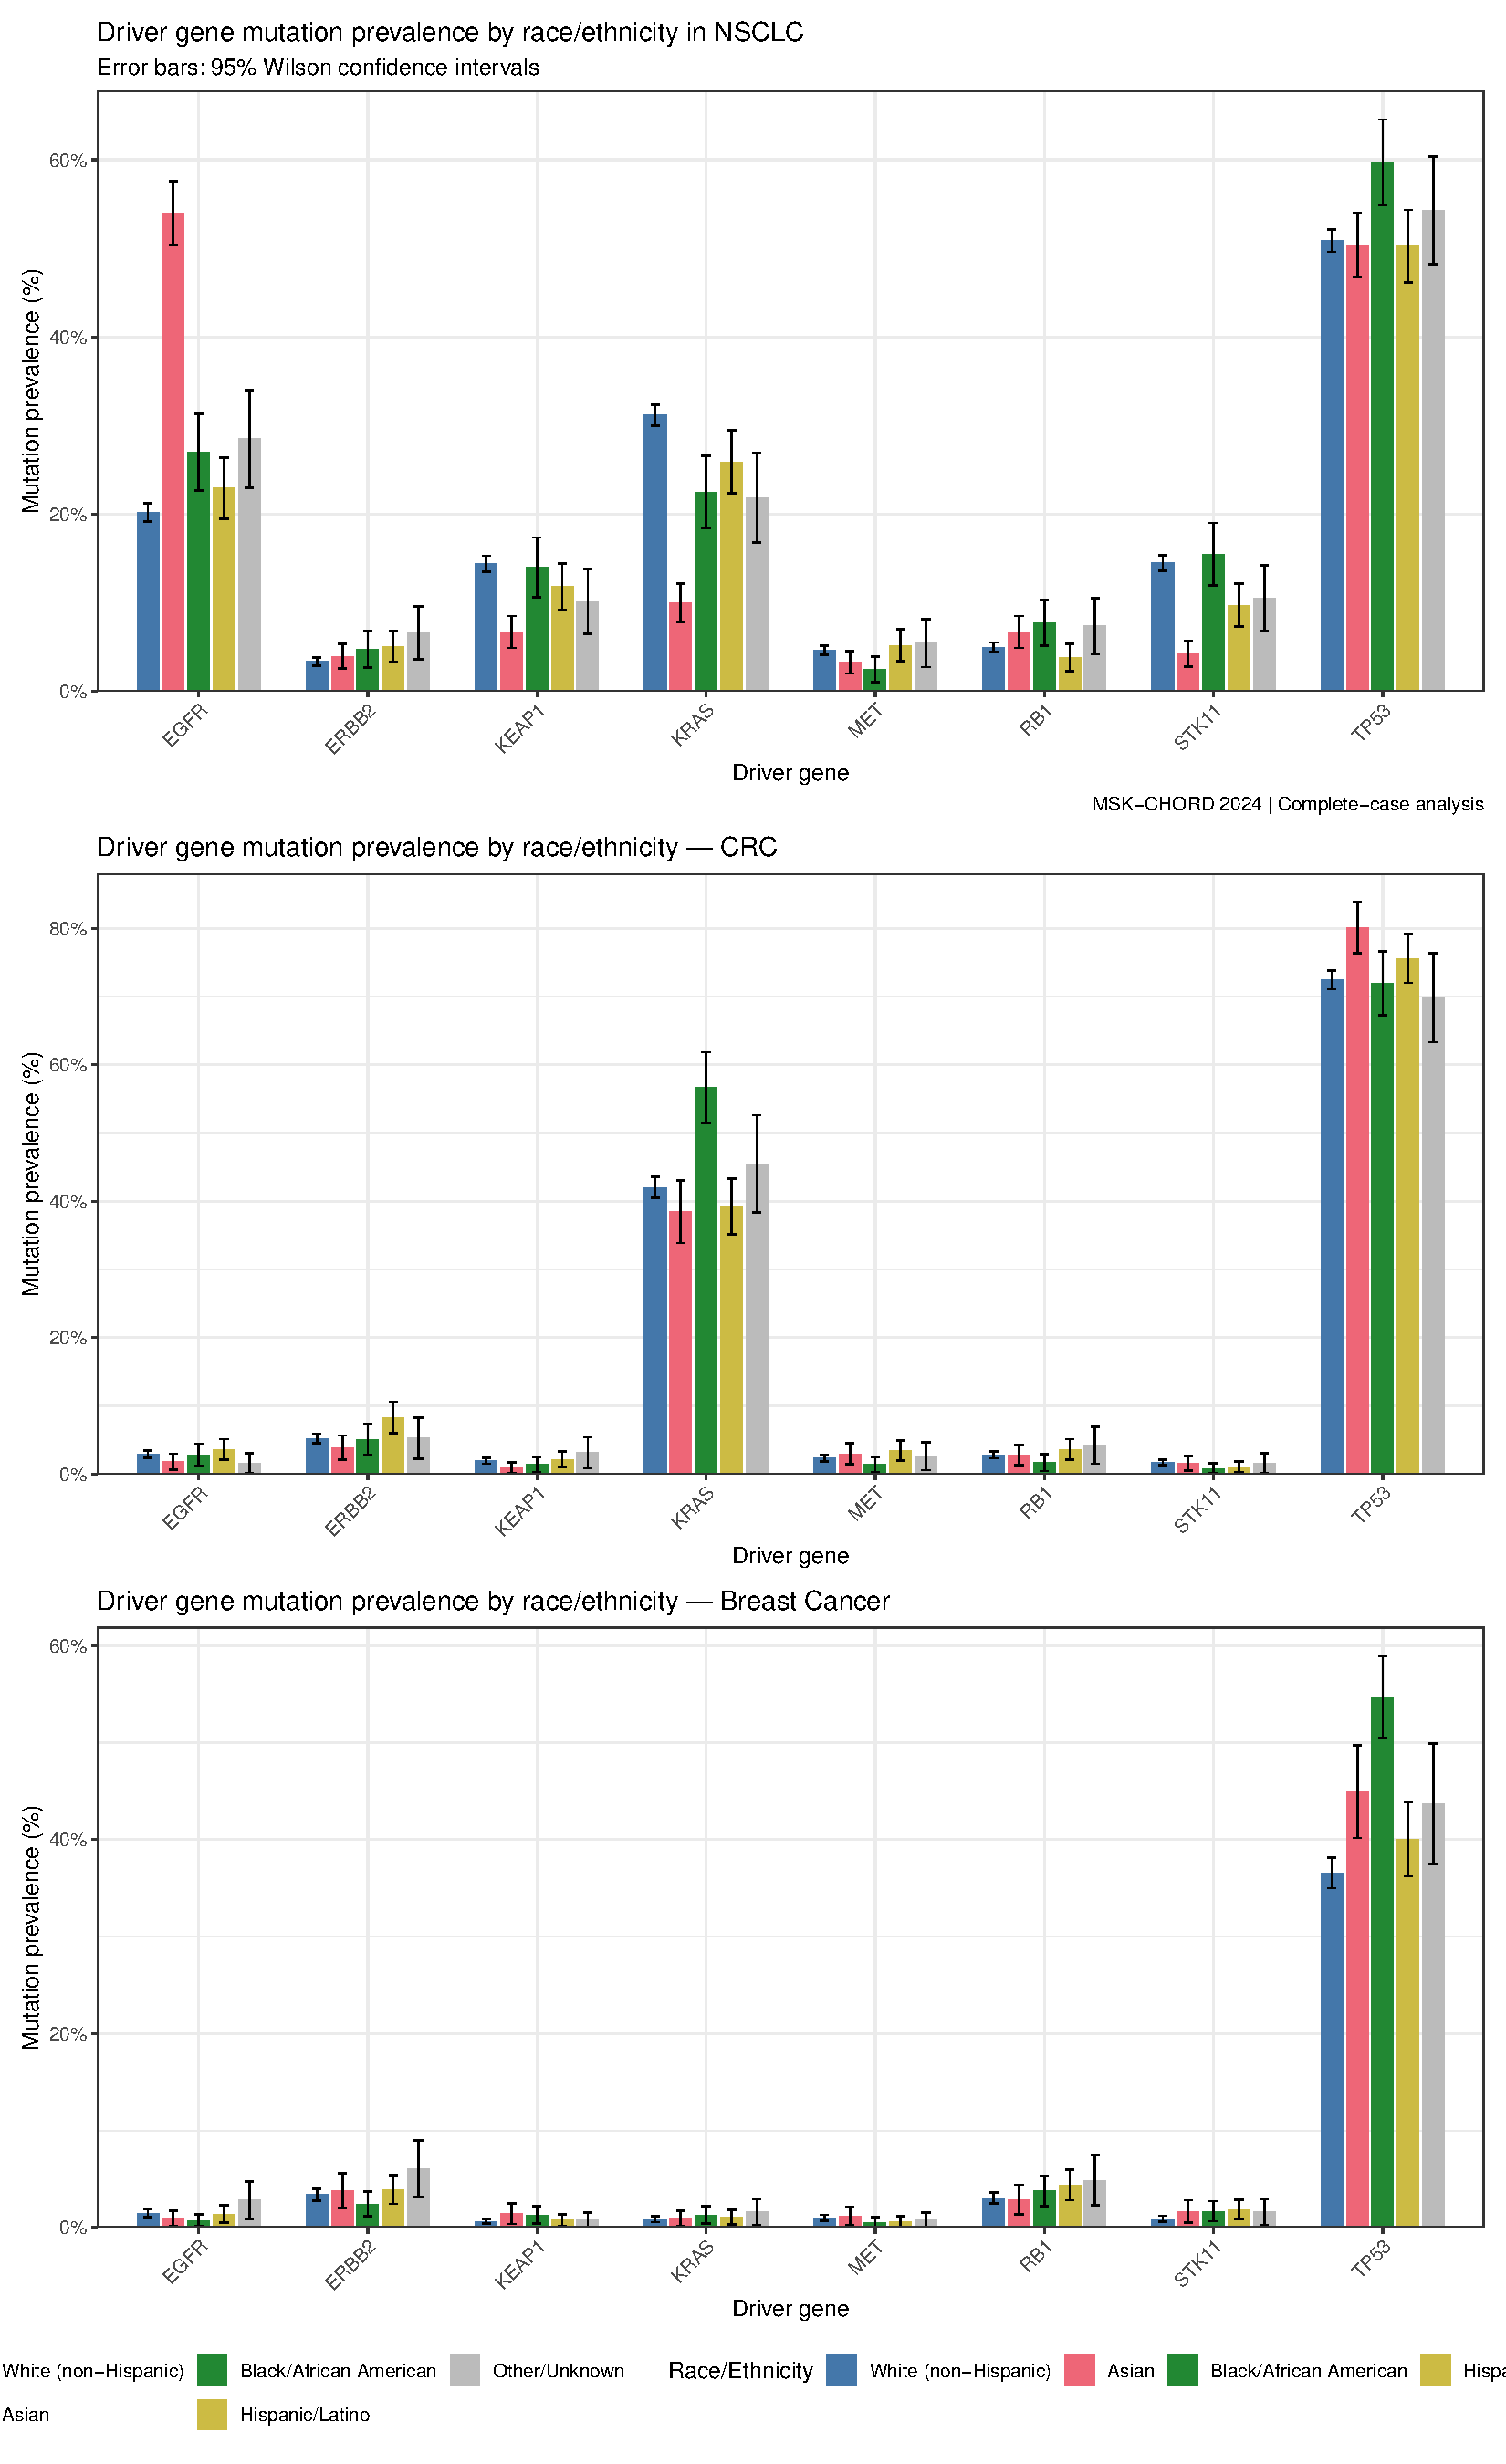
\includegraphics[width=\textwidth]{02_mutation_prevalence_all_cohorts.pdf}
  \caption{Driver gene mutation prevalence by race/ethnicity in NSCLC
           ($n = 7{,}775$).
           Error bars represent 95\% Wilson confidence intervals.
           EGFR shows the largest between-group disparity: Asian patients carry
           2.7~times the prevalence of White patients.
           KRAS and STK11 follow the reverse gradient.}
  \label{fig:prev}
\end{figure}

\subsection{Multivariable Logistic Regression}

After controlling for smoking history, disease stage, histologic subtype, sex,
and age, Asian patients retained 2.93~times the odds of EGFR mutation
compared with White patients (95\% CI 2.43--3.53, $q < 0.001$).
Asian patients showed less than half the odds of KRAS mutation
(adj.~OR 0.47, 95\% CI 0.36--0.62) and less than 40\% of the odds of STK11
mutation (adj.~OR 0.38, 95\% CI 0.25--0.57) compared with White patients.
Black patients showed a modestly elevated unadjusted EGFR rate, but the
difference did not reach significance after adjustment
(adj.~OR 1.25, 95\% CI 0.96--1.62, $q = 0.24$).
These results support H2: the EGFR and KRAS/STK11 race-mutation associations
are not explained by differential smoking exposure or stage at diagnosis.

\subsection{Survival Analysis}

EGFR-mutant patients had a median OS of 48.4~months versus 36.3~months for
wild-type patients (log-rank $p < 0.001$; Figure~\ref{fig:km}).
In the multivariable Cox model, EGFR mutation was independently associated with
improved survival (HR 0.82, 95\% CI 0.74--0.91, $p < 0.001$) after adjusting
for race/ethnicity, smoking, stage, sex, and age.
Stage~IV carried the strongest prognostic effect
(HR 2.88, 95\% CI 2.68--3.08, $p < 10^{-195}$).
The Race\,$\times$\,EGFR interaction terms did not reach statistical
significance for any racial group (all FDR-adjusted $p > 0.15$), which does
not support H3: EGFR enrichment in Asian patients does not translate to a
race-specific survival advantage in this cohort.
The proportional hazards assumption was satisfied for race, EGFR status, and
stage (Schoenfeld residual test $p > 0.10$ for all three).

\begin{figure}[H]
  \centering
  
\includegraphics[width=0.85\textwidth]{05_km_egfr_only.pdf}
  \caption{Kaplan-Meier overall survival curves by EGFR mutation status in
           NSCLC ($n = 7{,}775$).
           EGFR-mutant patients show longer median survival
           (48.4 vs.\ 36.3~months, log-rank $p < 0.001$).
           Numbers at risk are shown below the time axis.
           Shaded bands represent pointwise 95\% confidence intervals.}
  \label{fig:km}
\end{figure}

\subsection{Replication in CRC and Breast Cancer Cohorts}

Figure~\ref{fig:rep} shows adjusted ORs for EGFR across NSCLC, CRC, and
breast cancer.
EGFR enrichment in Asian patients reaches OR 2.93 in NSCLC but attenuates
toward the null in CRC (OR 0.39, 95\% CI 0.14--0.86) and reverses in breast
cancer (OR 0.35, 95\% CI 0.06--1.15).
This pattern supports H4: EGFR mutation enrichment in Asian patients is a
lung-tissue-specific phenomenon, not a pan-cancer racial genomic signal.
By contrast, TP53 enrichment in Black patients reaches significance in breast
cancer (adj.~OR 1.93, 95\% CI 1.59--2.34, $p = 3 \times 10^{-11}$) but not
in NSCLC (adj.~OR 1.36, 95\% CI 1.09--1.70, $q = 0.05$), suggesting
cancer-type-specific racial disparities for TP53.

\begin{figure}[H]
  \centering
  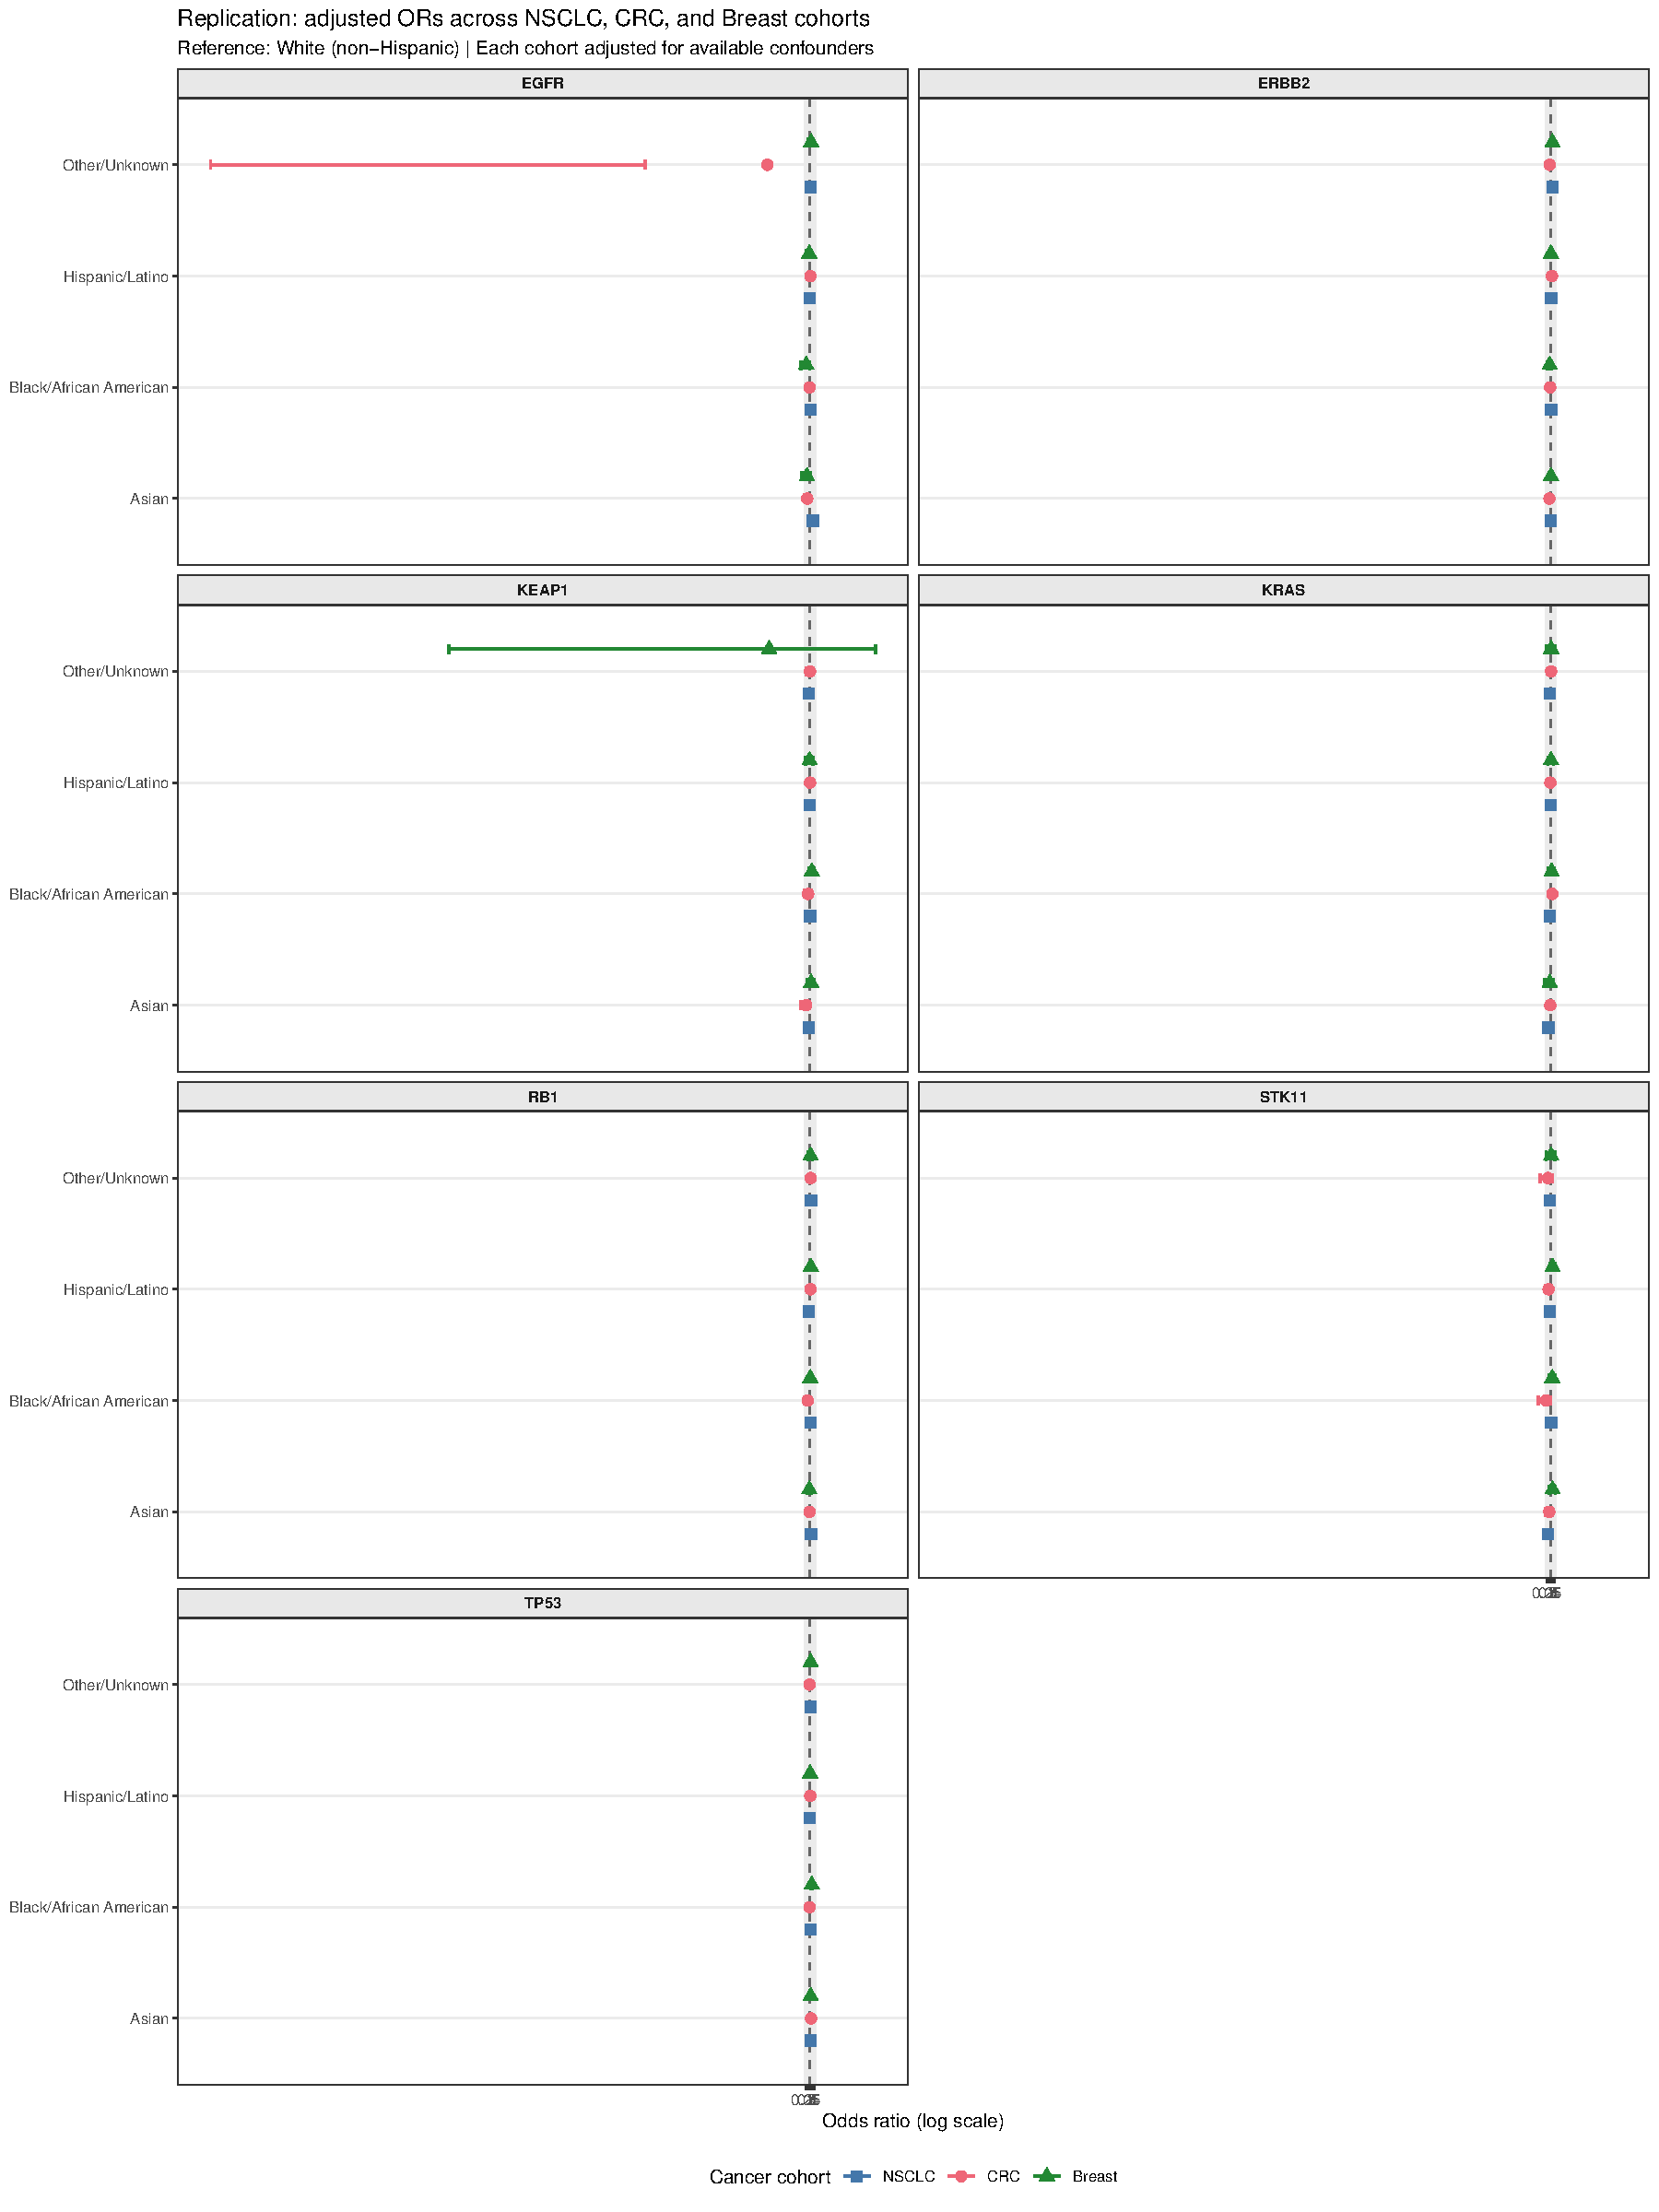
\includegraphics[width=\textwidth]{06_replication_forest_all_cohorts.pdf}
  \caption{Cross-cohort replication of adjusted ORs for EGFR and KRAS in
           Asian and Black patients.
           Reference group: White (non-Hispanic).
           EGFR enrichment in Asian patients (OR 2.93) is present only in
           NSCLC and attenuates sharply in CRC and breast cancer.
           Error bars represent 95\% confidence intervals.}
  \label{fig:rep}
\end{figure}

% =============================================================================
\section{Discussion}

This study confirms that EGFR mutation frequency in NSCLC differs markedly
across racial/ethnic groups and that this difference is not explained by
smoking history, disease stage, or histologic subtype.
Asian patients carry approximately three times the adjusted odds of EGFR
mutation compared with White patients, consistent with prior reports from East
Asian clinical trial populations \cite{Shigematsu2005}.
The replication analysis provides new evidence that this association is
lung-specific: EGFR enrichment disappears in CRC and breast cancer from the
same institution and sequencing platform, ruling out technical artifacts or
differential access to sequencing as the primary driver.

The Cox model supports EGFR mutation as a prognostic factor independent of
race (HR 0.82), but the Race\,$\times$\,EGFR interaction terms are
non-significant.
The survival benefit of EGFR-mutant patients therefore reflects the direct
effect of targeted therapy rather than a race-specific difference in tumour
biology or treatment response.
Black patients show the shortest median OS for EGFR wild-type tumours
(18.7~months), and this disadvantage persists after stage and smoking
adjustment---consistent with unmeasured barriers to TKI access or
comorbidity burden not captured in this dataset.

Three limitations constrain interpretation.
First, MSK-CHORD is drawn from a single tertiary cancer centre that
overrepresents commercially insured patients; results may not generalise to
community oncology settings.
Second, race and ethnicity are self-reported and collapsed into five broad
categories, obscuring within-group heterogeneity (EGFR mutation rates differ
between East Asian and South Asian patients).
Third, the analysis lacks germline sequencing data, so it cannot distinguish
somatic mutation frequencies from inherited predisposition to EGFR-activating
variants.

Lung-specific EGFR enrichment in Asian patients supports routine EGFR testing
at diagnosis for all Asian patients with NSCLC, regardless of smoking history.
Black patients' younger age at diagnosis and higher Stage~IV rate suggest
opportunities for earlier screening and intervention.
Future work should integrate population-level germline GWAS data to determine
what fraction of somatic EGFR enrichment is attributable to inherited variation,
and should examine whether TKI treatment rates fully mediate the
Race\,$\times$\,EGFR survival pattern observed here.

% =============================================================================
\begin{thebibliography}{9}

\bibitem{BH1995}
Benjamini~Y, Hochberg~Y.
Controlling the false discovery rate: a practical and powerful approach to
multiple testing.
\textit{J Royal Statistical Society Ser B.} 1995;57(1):289--302.

\bibitem{Cerami2012}
Cerami~E, Gao~J, Dogrusoz~U, et~al.
The cBio cancer genomics portal: an open platform for exploring
multidimensional cancer genomics data.
\textit{Cancer Discovery.} 2012;2(5):401--404.

\bibitem{Cohen1988}
Cohen~J.
\textit{Statistical Power Analysis for the Behavioral Sciences.}
2nd~ed. Erlbaum; 1988.

\bibitem{Mok2009}
Mok~TS, Wu~YL, Thongprasert~S, et~al.
Gefitinib or carboplatin-paclitaxel in pulmonary adenocarcinoma.
\textit{New England Journal of Medicine.} 2009;361(10):947--957.

\bibitem{Shigematsu2005}
Shigematsu~H, Lin~L, Takahashi~T, et~al.
Clinical and biological features associated with epidermal growth factor
receptor gene mutations in lung cancers.
\textit{Journal of the National Cancer Institute.} 2005;97(5):339--346.

\bibitem{Siegel2023}
Siegel~RL, Miller~KD, Wagle~NS, Jemal~A.
Cancer statistics, 2023.
\textit{CA: A Cancer Journal for Clinicians.} 2023;73(1):17--48.

\bibitem{vanBuuren2018}
van Buuren~S.
\textit{Flexible Imputation of Missing Data.}
2nd~ed. CRC Press; 2018.

\end{thebibliography}

\end{document}
